% providecommand redefines the command only if not already defined.
% This is useful to define a different path to other files for subfiles compared to the main thesis.
\providecommand{\main}{..} % Relative path of the main thesis (`..` represents the parent directory)
\providecommand{\figures}{\main/figures}

% The subfiles document class uses the preamble from the file in the optional argument. Don't repeat it.
\documentclass[\main/ExampleThesis]{subfiles}

\begin{document}

\unpacklipsum[141][1] % Unpack 1 sentence of lipsum text for use in the appendix title
\chapter{\lipsumexp}
\lipsum[140][4]

\begin{figure}[h]
  \centering
  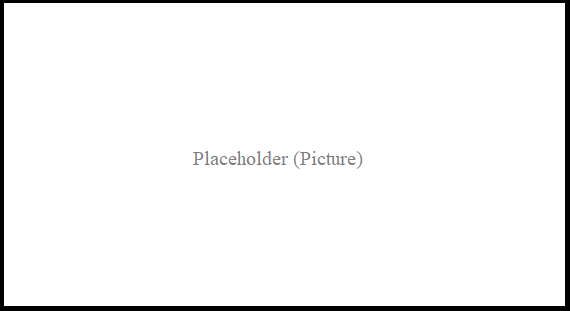
\includegraphics[width=0.5\textwidth]{figures/pictures/placeholder}
  \caption{The caption of the figure}
  \label{fig:placeholder4}
\end{figure}

\section{\lipsum[140][3]}
\lipsum[8-9]

\section{\lipsum[140][5]}
\lipsum[10]

\end{document}